\documentclass[10pt,journal,compsoc]{IEEEtran}

\usepackage[pdftex]{graphicx}    
\usepackage{cite}
\usepackage{hyperref}
\hyphenation{op-tical net-works semi-conduc-tor}


\begin{document}

\title{Robotics Inference}

\author{Ghee Chong Foo}

\markboth{Inference project, Robotic Nanodegree, Udacity}%
{}
\IEEEtitleabstractindextext{%

\begin{abstract}

This write up is about robotics inferencing utilizing NVIDIA's DIGITS (Deep Learning GPU Training System) for both supplied and own data. For supplied data, 3 class of objects (bottle, candy and nothing) with images provided by Udacity will be inferred and results benchmarked against inference time and accuracy.  For own data, a clothing classification model was presented.  Only 3 class of clothing, namely shorts, shirts and long sleeve shirt are attempted.  The prototype was able to infer new images with accuracy $>$ 90\% for own datasets, but performed with varied accuracy with data source from Internet.

\end{abstract}

% Note that keywords are not normally used for peerreview papers.
\begin{IEEEkeywords}
Robotics, deep learning, inference.
\end{IEEEkeywords}}


\maketitle
\IEEEdisplaynontitleabstractindextext
\IEEEpeerreviewmaketitle
\section{Introduction}
\label{sec:introduction}

\IEEEPARstart
In this section the motivation for both supplied and own data will be discussed.

\subsection{Supplied Data}
The first part of project was to train supplied data that consist of color images of "bottle", "candy" and "nothing" on a conveyor belt, potentially for sorting purposes in manufacturing packing station.  The idea can be generalize to all kinds of items that fit on a conveyor belt, and when the desired item is detected, a mechanism can be activated to trigger the item to be dropped to desired container(s).\linebreak

\subsection{Own Data}
The second part of the project was to come up with own idea for robotics inferencing. A clothing identification project was inspired to resolve a day to day chore, i.e. cloth folding.  While washing machines has been in existence for decades and a great relief for homemakers from having to perform mundane laundry work, the subsequent step of folding the cleaned laundry, is still have to be done by hand/human, as the seemingly simple procedure of recognizing type of clothing and how to fold it, is still a task too daunting to be handled by machines.  \linebreak 

The purpose of this part is to solve the first stage of cloth folding problem, i.e. classifying the type of cloth before subsequent logic will handle the actual folding part.  It should be noted that in recent CES 2018, a company called "Seven Dreamers" has come up with similar ideas\cite{theverge}, namely "Laundroid", indicating a huge unsatisfied market for this application.

% {T}{he} introduction should provide some material regarding the history of the problem, why it is important and what is intended to be achieved. If there exists any previous attempts to solve this problem, this is a great place to note these while conveying the differences in your approach (if any). The intent is to provide enough information for the reader to understand why this problem is interesting and setting up the conversation for the solution you have provided
% Use this space to introduce your robotic inference idea and how you wish to apply it. 
% If you have any papers / sites you have referenced for your idea, please make sure to cite them.

% \begin{table}[h]
% \caption{Table}
% \label{table_example}
% \begin{center}
% \begin{tabular}{|c||c|}
% \hline
% One & Two\\
% \hline
% Three & Four\\
% \hline
% \end{tabular}
% \end{center}
% \end{table}

\section{Background / Formulation}
In this project NVIDIA"s DIGITS was deployed to utilize state of the art GPU in the cloud to prototype image processing ideas.  By using data that are commonly used for image processing training (e.g. MNIST), or uploading own data, one can test out the model quickly after training the model with standard network (e.g. LeNET, AlexNET or GoogLeNet), or train with a customized model. \linebreak

For this project, since the data consist of color images for both supplied and own data, it will be trained against AlexNet and GooLeNet which are optimized for color images. The hyperparameters are then adjusted by observing the loss curve for final validation accuracy, as well as trending of training loss vs. validation loss, to achieve desired result.\linebreak

The following parameters was found to be optimum for this project (Table ~\ref{hyperparameter}), with the other entries left as default:

% \begin{itemize}
% \item Training Epochs: 10
% \item Batch size: 25
% \item Solver type: SGD (Stochastic Gradient Descent)
% \item Learning rate: 0.001
% \end {itemize}

\begin{table}[!htbp]
\caption{Hyperparameter}
\label{hyperparameter}
\begin{center}
\begin{tabular}{|c||c|}
\hline
Training Epochs & 10(supplied data)/30(own data)\\
\hline
Batch size & 25\\
\hline
Solver type & SGD (Stochastic Gradient Descent)\\
\hline
Image type & RGB\\
\hline
Learning rate & 0.001\\
\hline
\end{tabular}
\end{center}
\end{table}


It was found that adjusting the hyperparameters alone was not sufficient to achieve the goal, and one might need to recollect the data/images with proper settings, this will be discussed further in \textit{Discussion} section.

% At this stage, you should begin diving into the technical details of your approach by explaining to the reader how parameters were defined, what type of network was chosen, and the reasons these items were performed. This should be factual and authoritative, meaning you should not use language such as “I think this will work” or “Maybe a network with this architecture is better..”. Instead, focus on items similar to, ”A 3-layer network architecture was chosen with X, Y, and Z parameters” 
% Explain why you chose the network you did for the supplied data set and then why you chose the network used for your robotic inference project. \cite{journals/corr/ZeilerF13}

% %example for Bullet point list

% \begin{itemize}
% \item example
% \end {itemize}

%example for numbered list
% \begin{enumerate}
% \item example
% \end{enumerate}

\section{Data Acquisition}
\subsection{Supplied Data}

A data set was provided by Udacity with as shown in Table ~\ref{supplied data set details}:
\begin{table}[h]
\caption{Supplied Data Set Details}
\label{supplied data set details}
\begin{center}
\begin{tabular}{|c||c|}
\hline
Images category & Groceries\\
\hline
Number of Images & 10100\\
\hline
Image size & 500x500\\
\hline
Image type & RGB\\
\hline
Number of class & 3\\
\hline
Image label & Bottle, Candy Box, Nothing\\
\hline
\end{tabular}
\end{center}
\end{table}

Sample supplied data was depicted in Fig. ~\ref{fig:Bottle}, ~\ref{fig:Candy} and ~\ref{fig:Nothing}.
%Insert supplied data image here
\begin{figure}[!htbp]
      \centering
      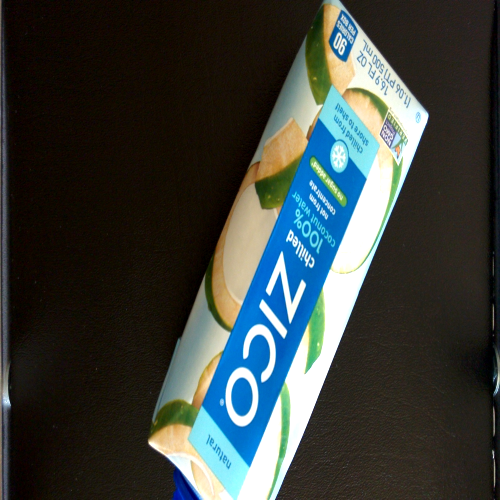
\includegraphics[width=0.3\textwidth]{coconut}
      \caption{Bottle (Supplied Data)}
      \label{fig:Bottle}
\end{figure}

\begin{figure}[!htbp]
      \centering
      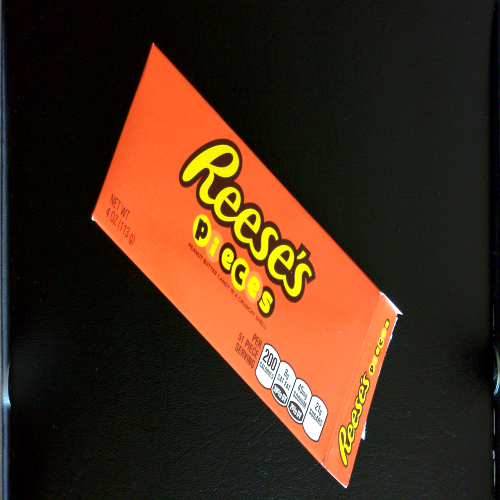
\includegraphics[width=0.3\textwidth]{reeses}
      \caption{Candy (Supplied Data)}
      \label{fig:Candy}
\end{figure}

\begin{figure}[!htbp]
      \centering
      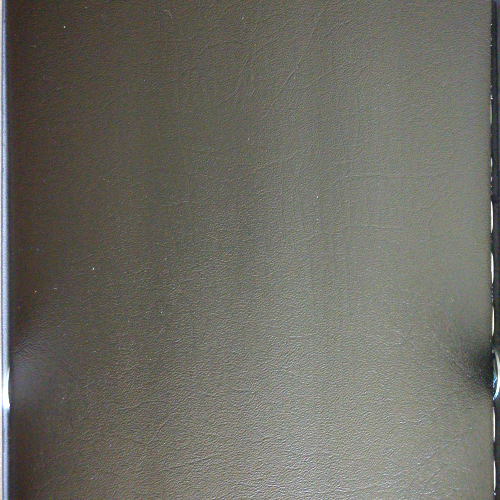
\includegraphics[width=0.3\textwidth]{Nothing}
      \caption{Nothing (Supplied Data)}
      \label{fig:Nothing}
\end{figure}

\subsection{Own Data}

Own data was captured using smartphone (an iPhone 8 Plus) and placing the camera at fixed height so as to preserve the relative size of the objects.  Images was captured in well lit room with natural light.  Sample of own data was depicted in Fig. ~\ref{fig:Shorts}, ~\ref{fig:Long_sleeve} and ~\ref{fig:Socks}.

Details of own data set was outlined as Table ~\ref{own data set details} below:
\begin{table}[!htbp]
\caption{Own Data Set Details}
\label{own data set details}
\begin{center}
\begin{tabular}{|c||c|}
\hline
Images category & Clothing\\
\hline
Number of Images & 1631\\
\hline
Image size & 360x480\\
\hline
Image type & RGB\\
\hline
Number of class & 3\\
\hline
Image label & Long Sleeves, Shorts, Socks\\
\hline
\end{tabular}
\end{center}
\end{table}

%Insert own data image here
\begin{figure}[!htbp]
      \centering
      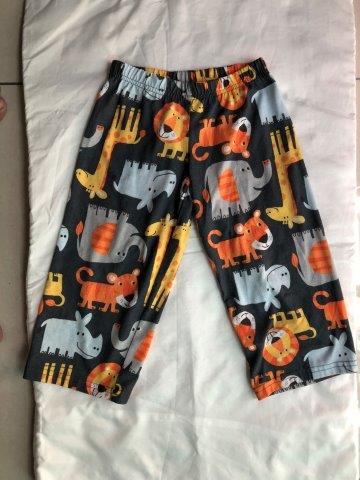
\includegraphics[width=0.25\textwidth]{Shorts}
      \caption{Shorts}
      \label{fig:Shorts}
\end{figure}

\begin{figure}[!htbp]
      \centering
      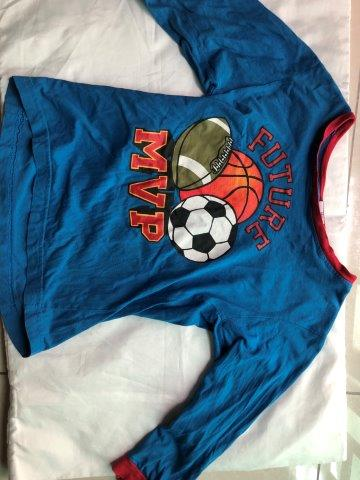
\includegraphics[width=0.25\textwidth]{Long_sleeve}
      \caption{Long Sleeve}
      \label{fig:Long_sleeve}
\end{figure}


\begin{figure}[!htbp]
      \centering
      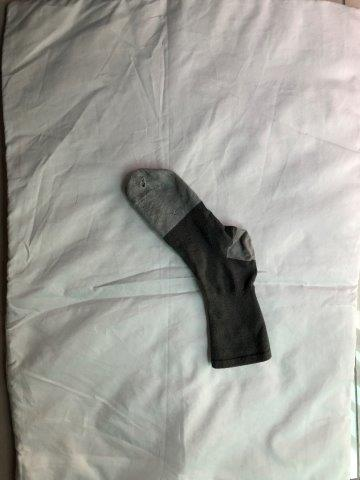
\includegraphics[width=0.25\textwidth]{Socks}
      \caption{Socks}
      \label{fig:Socks}
\end{figure}
% This section should discuss the data set. Items to include are the number of images, size of the images, the types of images (RGB, Grayscale, etc.), how these images were collected (including the method). Providing this information is critical if anyone would like to replicate your results. After all, the intent of reports such as these are to convey information and build upon ideas so you want to ensure others can validate your process.
% Justifying why you gathered data in this way is a helpful point, but sometimes this may be omitted here if the problem has been stated clearly in the introduction.
% It is a great idea here to have at least one or two images showing what your data looks like for the reader to visualize.

\newpage
\section{Results}
The inference results are discussed for both supplied data and own data.  In particular the results of training with AlexNet and GoogLeNet are compared for supplied data.

\subsection{Supplied Data}
\subsubsection{AlexNet}
When trained with AlexNet, there presents a steady drop of validation/training loss, with final accuracy of 98.53\% (Fig. ~\ref{fig:Alex_Epoch10_Batch25_lr001}).  The validation loss tracks the training loss closely, which suggest a good fit.  The model yielded run time of 8 minutes, 56 seconds for 10 epochs.
%Insert loss diagram here
\begin{figure}[thpb]
      \centering
      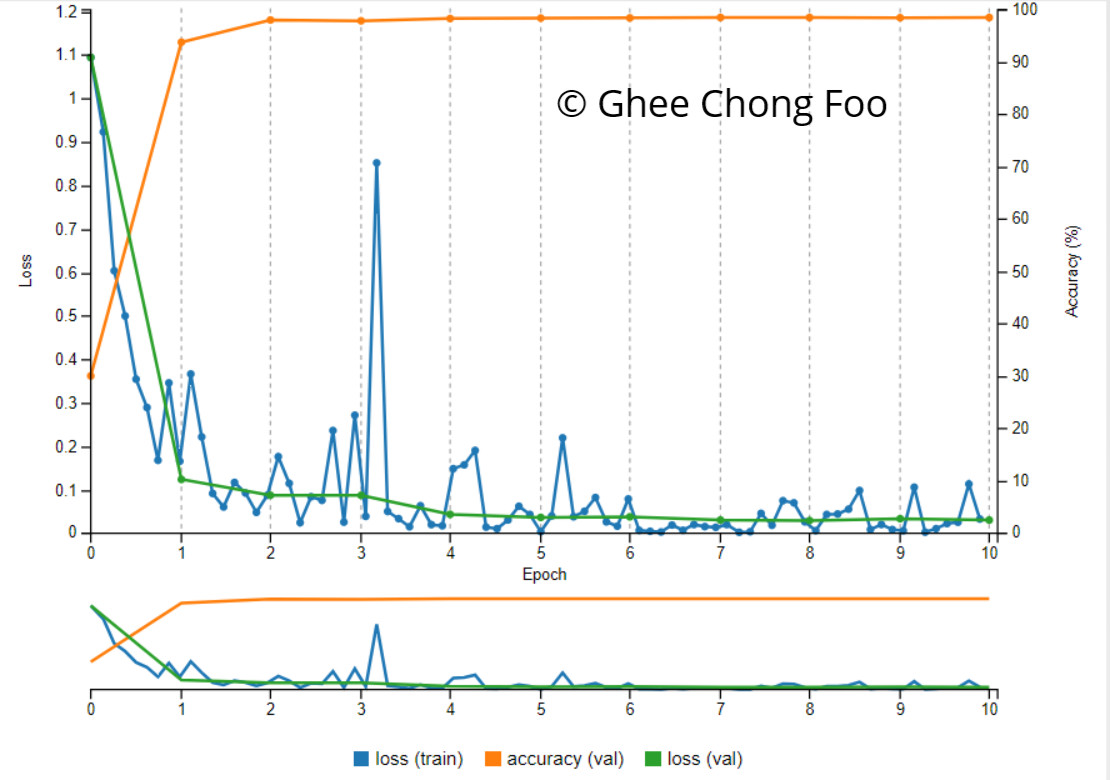
\includegraphics[width=\linewidth]{Alex_Epoch10_Batch25_lr001}
      \caption{AlexNet Loss Curve}
      \label{fig:Alex_Epoch10_Batch25_lr001}
\end{figure}

When the model ran through "evaluate" command, it return inference time of 4.199 milliseconds with accuracy of 75.41\% (Fig. ~\ref{fig:evaluate_AlexNet}), which meets project specification.

\begin{figure}[thpb]
      \centering
      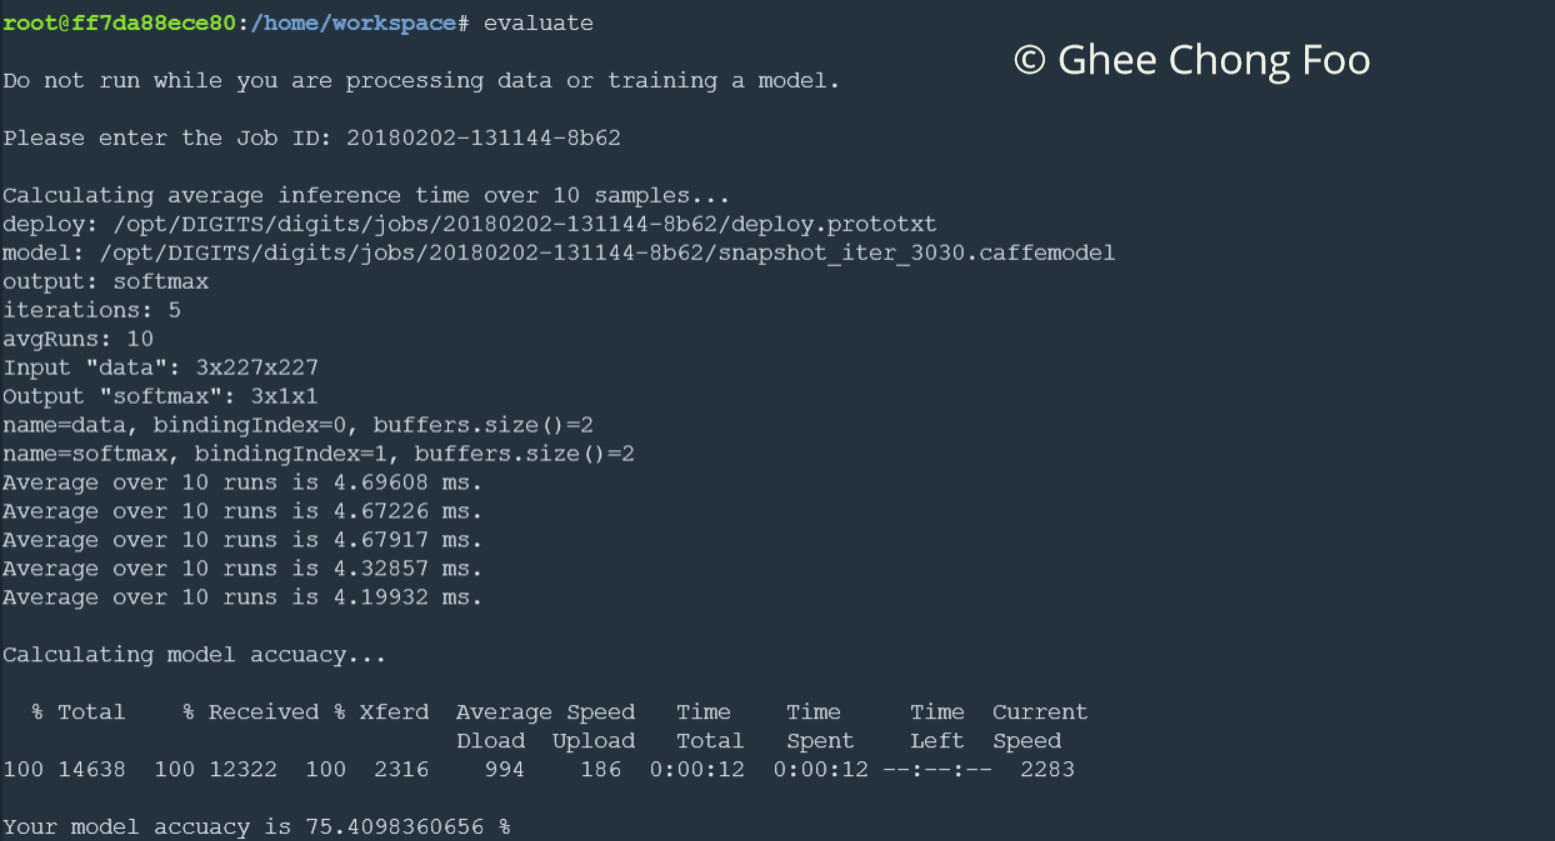
\includegraphics[width=\linewidth]{evaluate_AlexNet}
      \caption{Evaluate result for supplied data using AlexNet}
      \label{fig:evaluate_AlexNet}
\end{figure}

\subsubsection{GoogLeNet}
When the data set was trained with GoogLeNet, similar pattern was shown, with validation loss tracking training loss very closely.  Training yielded run time of 20 minutes, 8 seconds with accuracy of 99.8\% (Fig. ~\ref{fig:Goog_Epoch10_Batch25_lr001}).

\begin{figure}[thpb]
      \centering
      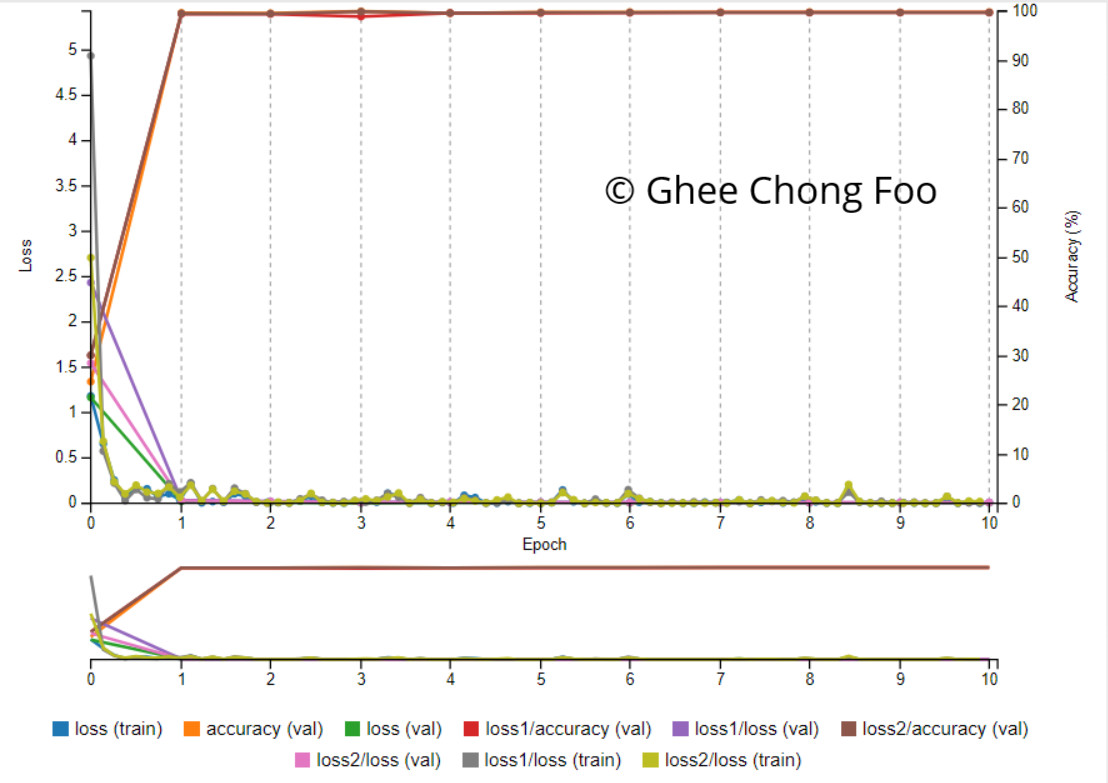
\includegraphics[width=\linewidth]{Goog_Epoch10_Batch25_lr001}
      \caption{GoogLeNet Loss Curve}
      \label{fig:Goog_Epoch10_Batch25_lr001}
\end{figure}

Running the GoogLeNet model through "evaluate" command, yielded inference time of 5.03 milliseconds and acurracy of 75.41\% (Fig. ~\ref{fig:evaluate_GooLeNet}), also meeting project specification.

\begin{figure}[thpb]
      \centering
      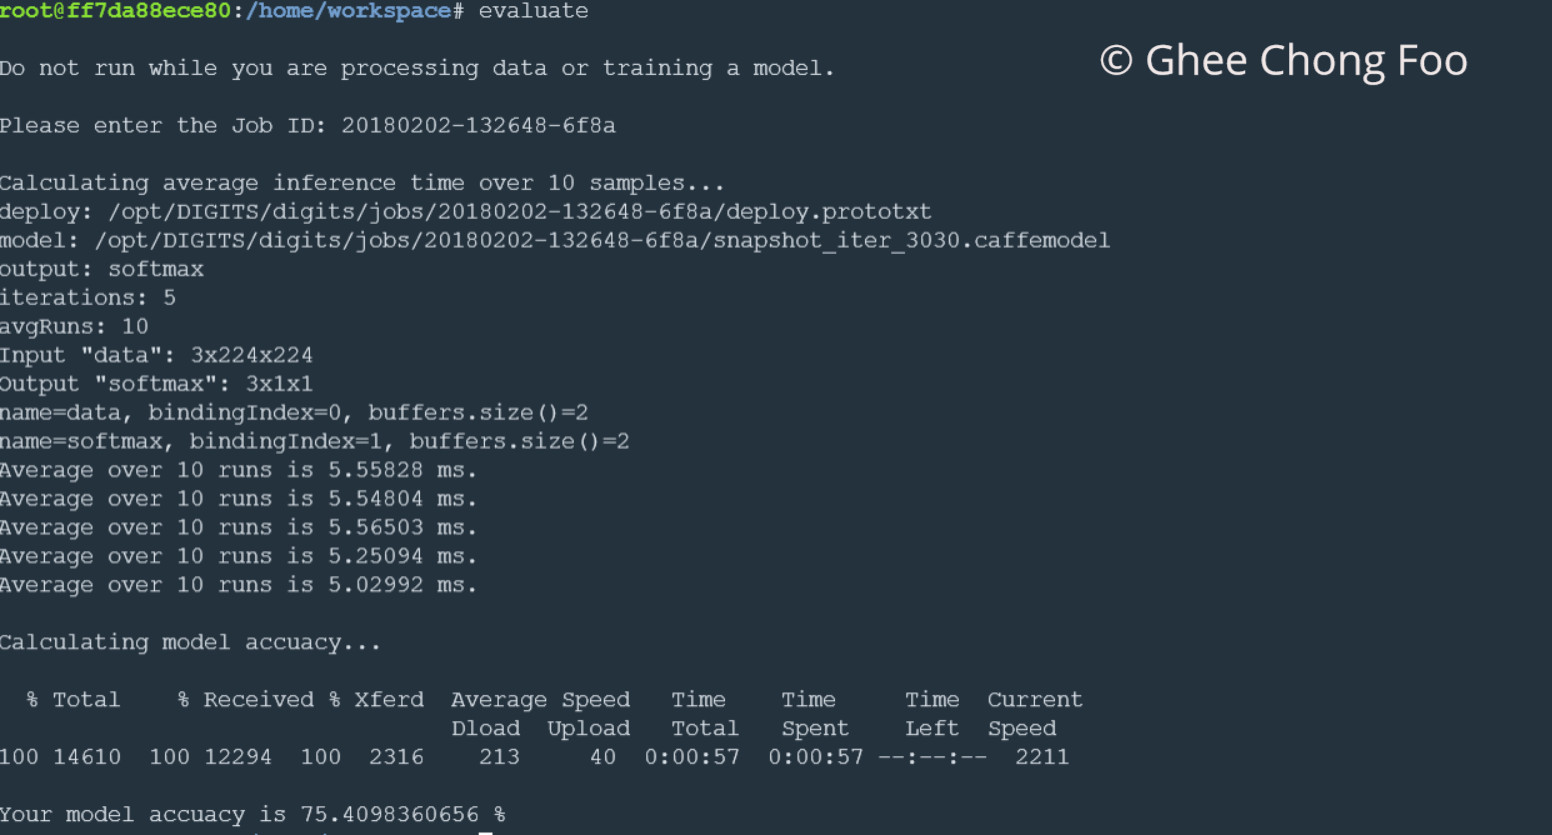
\includegraphics[width=\linewidth]{evaluate_GooLeNet}
      \caption{Evaluate result for supplied data using GoogLeNet}
      \label{fig:evaluate_GooLeNet}
\end{figure}

\subsection{Own Data}
Since AlexNet trains faster with comparable accuracy, only AlexNet was used to train the model for own data.  Training loss trend validation loss closely, with accuracy reaching 99.53\% in 4 minutes, 14 seconds (Fig. ~\ref{fig:loss_curve_clothing}).\linebreak

\begin{figure}[thpb]
      \centering
      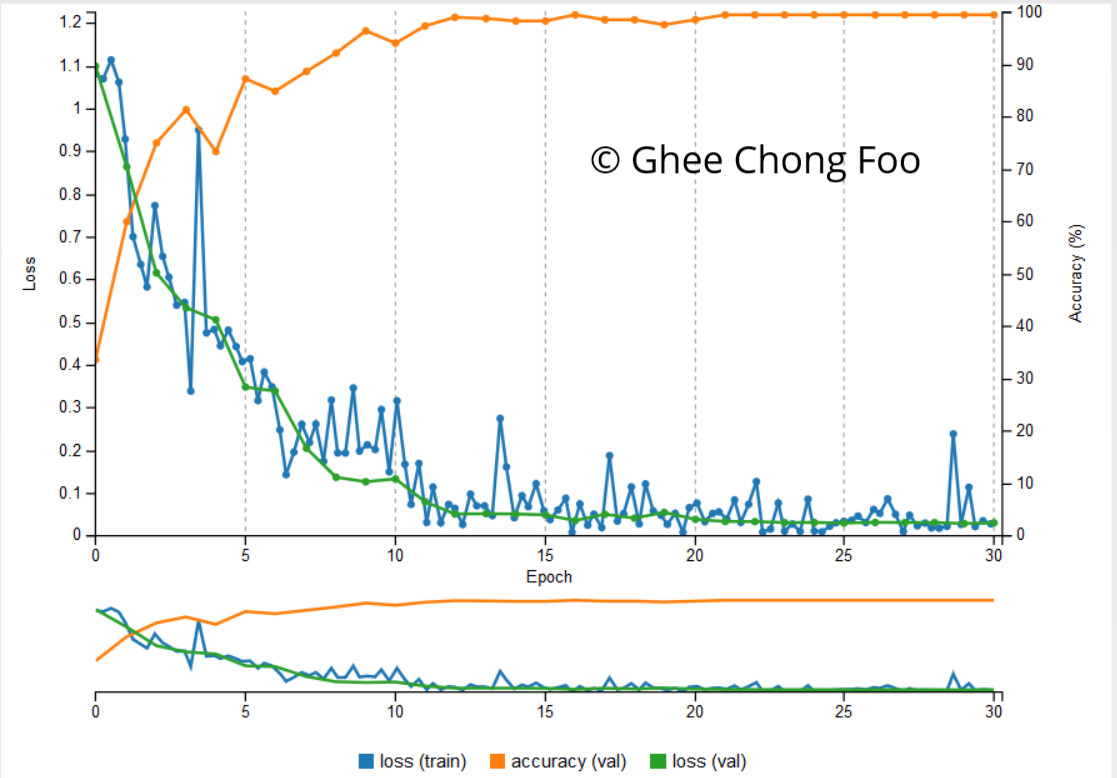
\includegraphics[width=\linewidth]{loss_curve_clothing}
      \caption{AlexNet Loss Curve for Clothing Model}
      \label{fig:loss_curve_clothing}
\end{figure}

The trained model was then asked to classify 9 images (3 each for every categories).  By using own collected data that has not been used for training, the model was able to correctly classifying 4 out of 5 images with $>$ 90\% possibilities in general. Using images from the Internet, the model can only correctly classify 1 out of 4 images, with 98.25\% probabilities for this particular object (Fig. ~\ref{fig:classify_many_clothing}).\linebreak

Sample of classifying one image output is shown in Fig. ~\ref{fig:long_bad_predict1}, ~\ref{fig:long_good_predict1}, ~\ref{fig:short_bad_predict1}, ~\ref{fig:short_bad_predict2}, ~\ref{fig:socks_bad_predict1}, ~\ref{fig:socks_good_predict1}.

\begin{figure}[thpb]
      \centering
      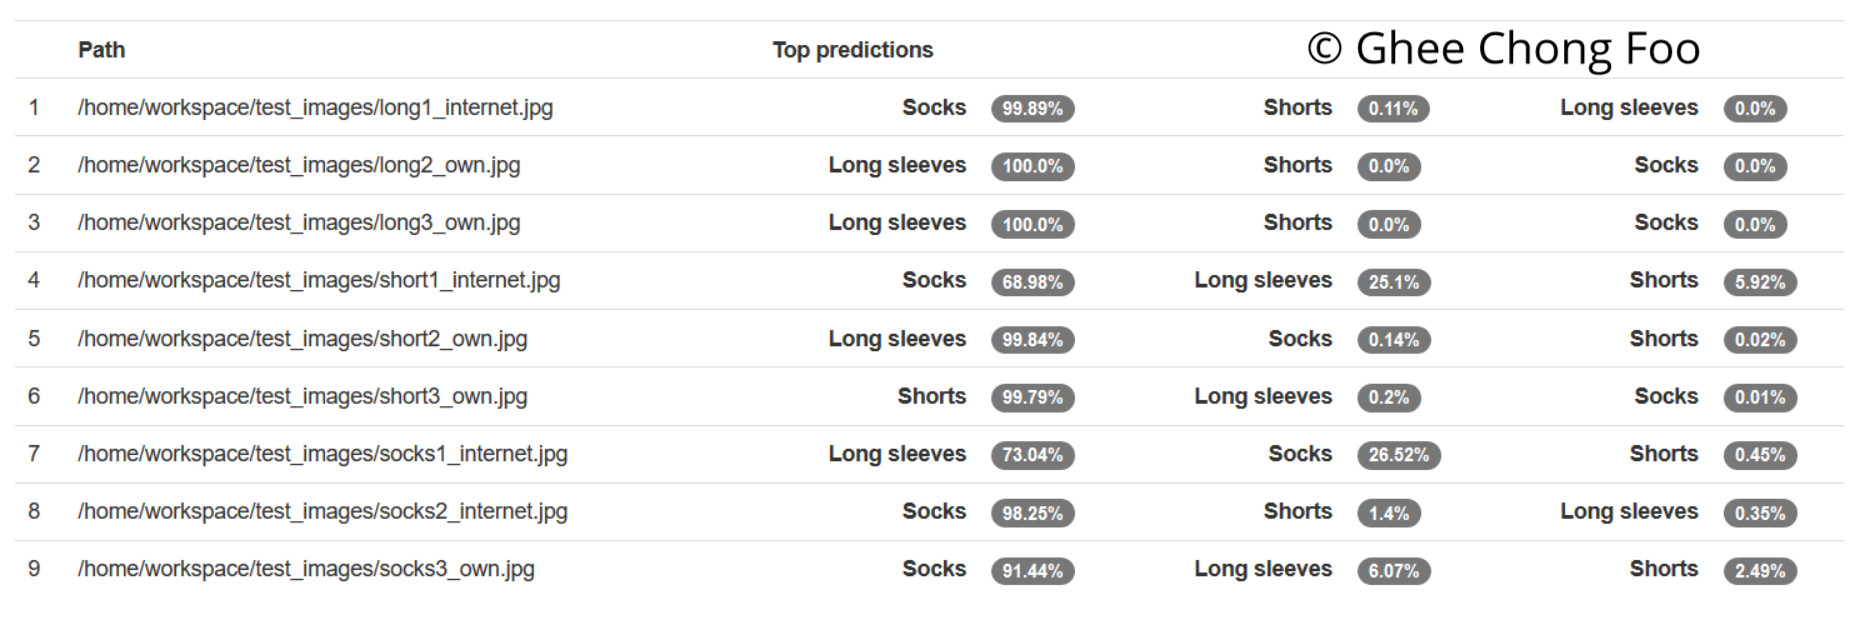
\includegraphics[width=\linewidth]{classify_many_clothing}
      \caption{Classification result}
      \label{fig:classify_many_clothing}
\end{figure}

\begin{figure}[thpb]
      \centering
      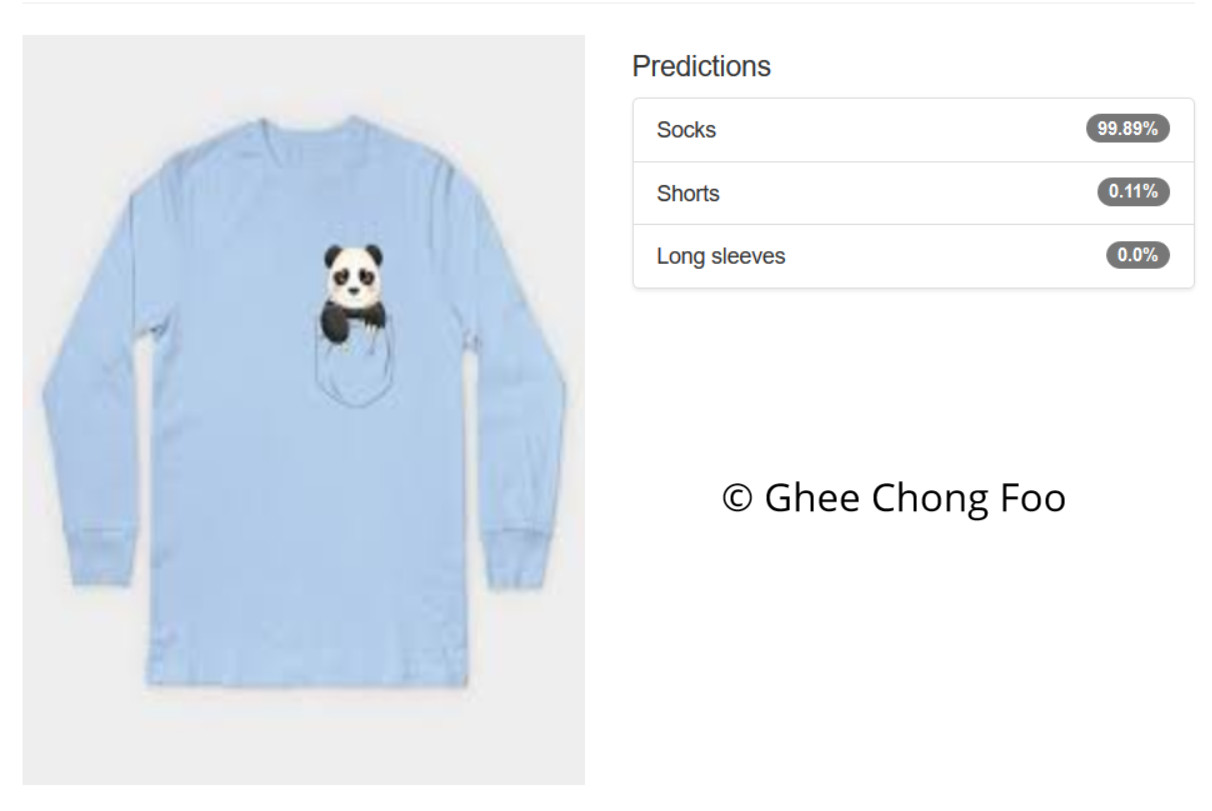
\includegraphics[width=\linewidth]{long_bad_predict1}
      \caption{Bad prediction for "Long sleeves" using Internet image}
      \label{fig:long_bad_predict1}
\end{figure}

\begin{figure}[thpb]
      \centering
      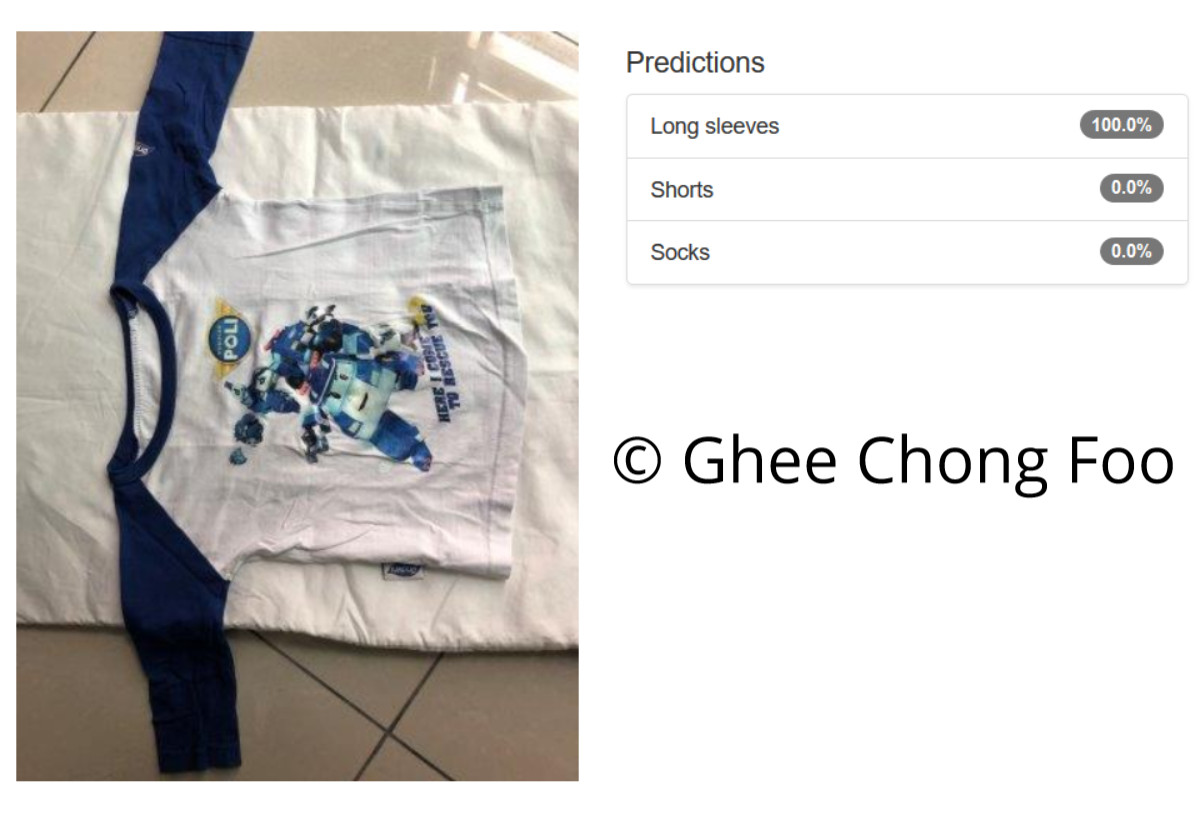
\includegraphics[width=\linewidth]{long_good_predict1}
      \caption{Good prediction for "Long sleeves" using own data}
      \label{fig:long_good_predict1}
\end{figure}

\begin{figure}[thpb]
      \centering
      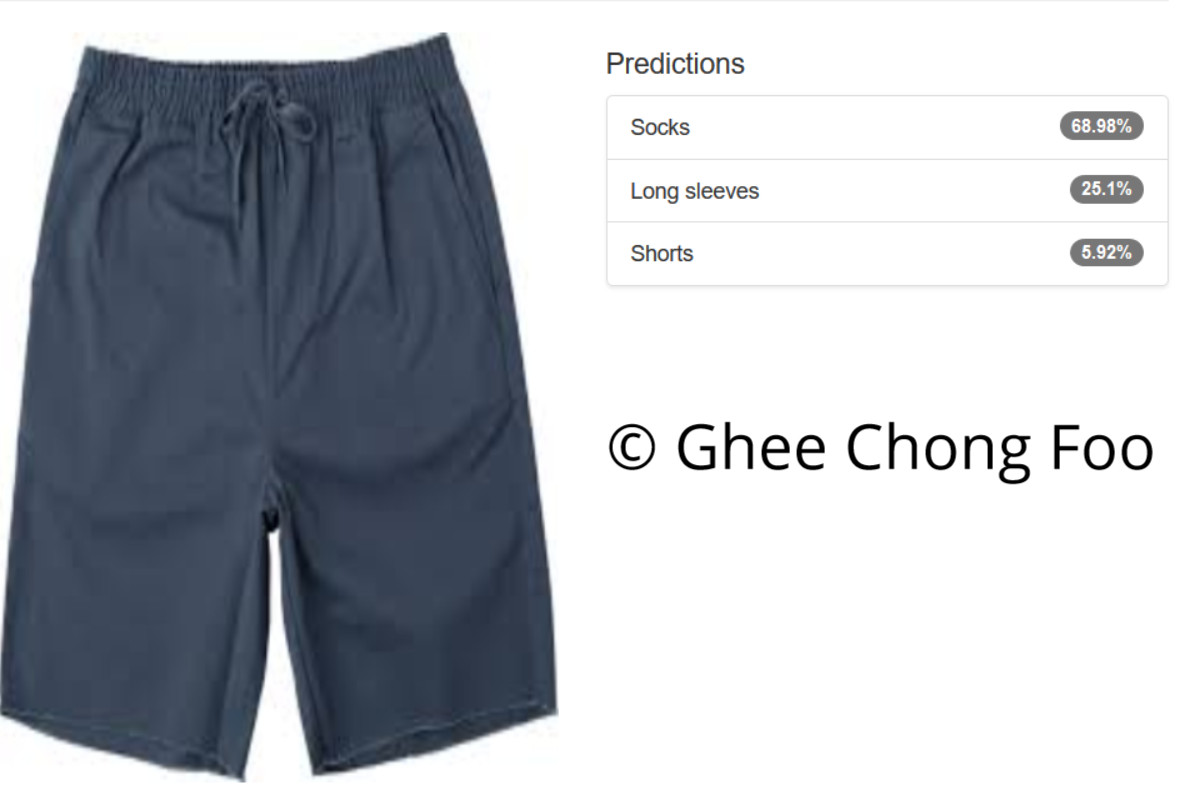
\includegraphics[width=\linewidth]{short_bad_predict1}
      \caption{Bad prediction for "Shorts" using Internet image}
      \label{fig:short_bad_predict1}
\end{figure}

\begin{figure}[thpb]
      \centering
      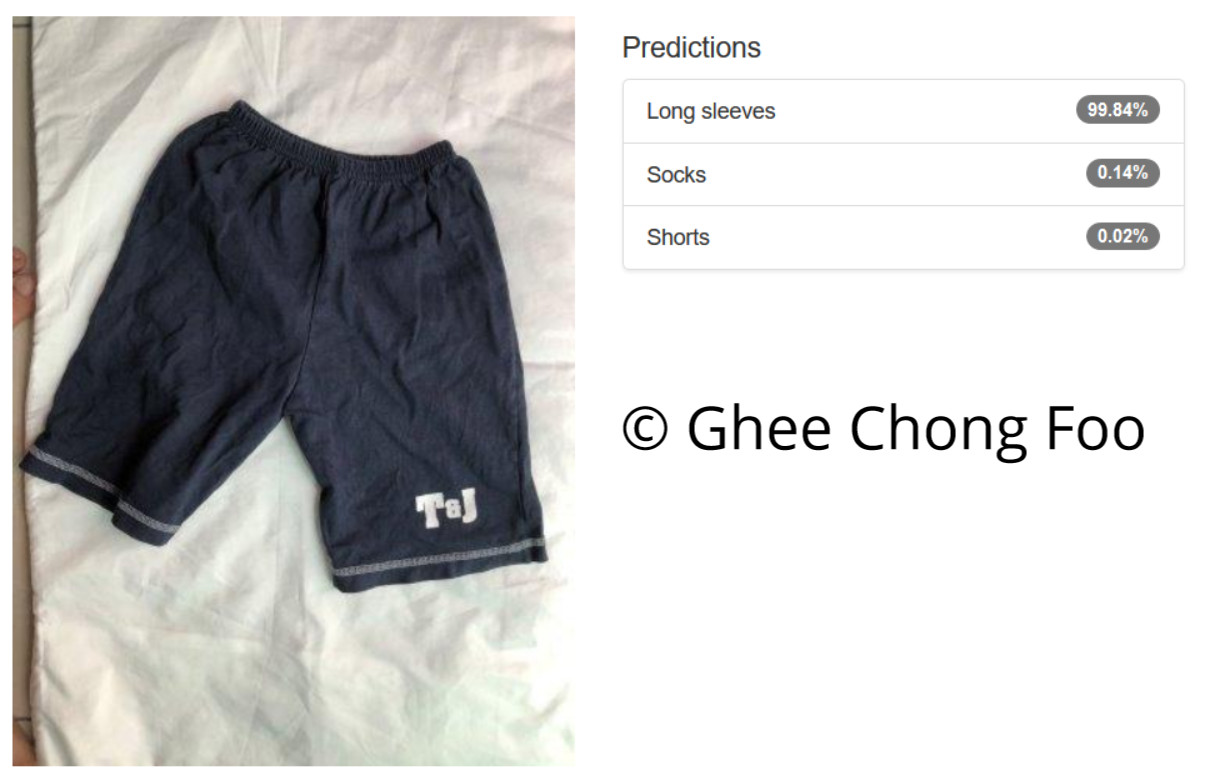
\includegraphics[width=\linewidth]{short_bad_predict2}
      \caption{Bad prediction for "Shorts" using own data}
      \label{fig:short_bad_predict2}
\end{figure}

\begin{figure}[thpb]
      \centering
      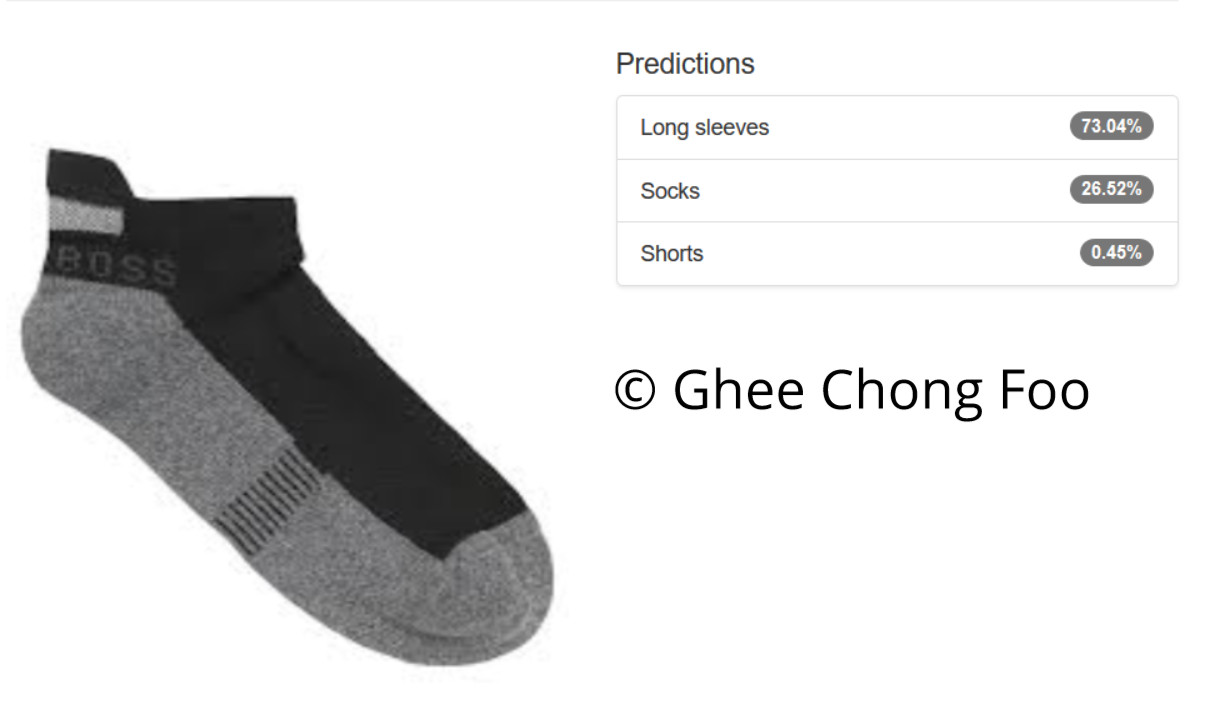
\includegraphics[width=\linewidth]{socks_bad_predict1}
      \caption{Bad prediction for "Socks" using Internet image}
      \label{fig:socks_bad_predict1}
\end{figure}

\begin{figure}[thpb]
      \centering
      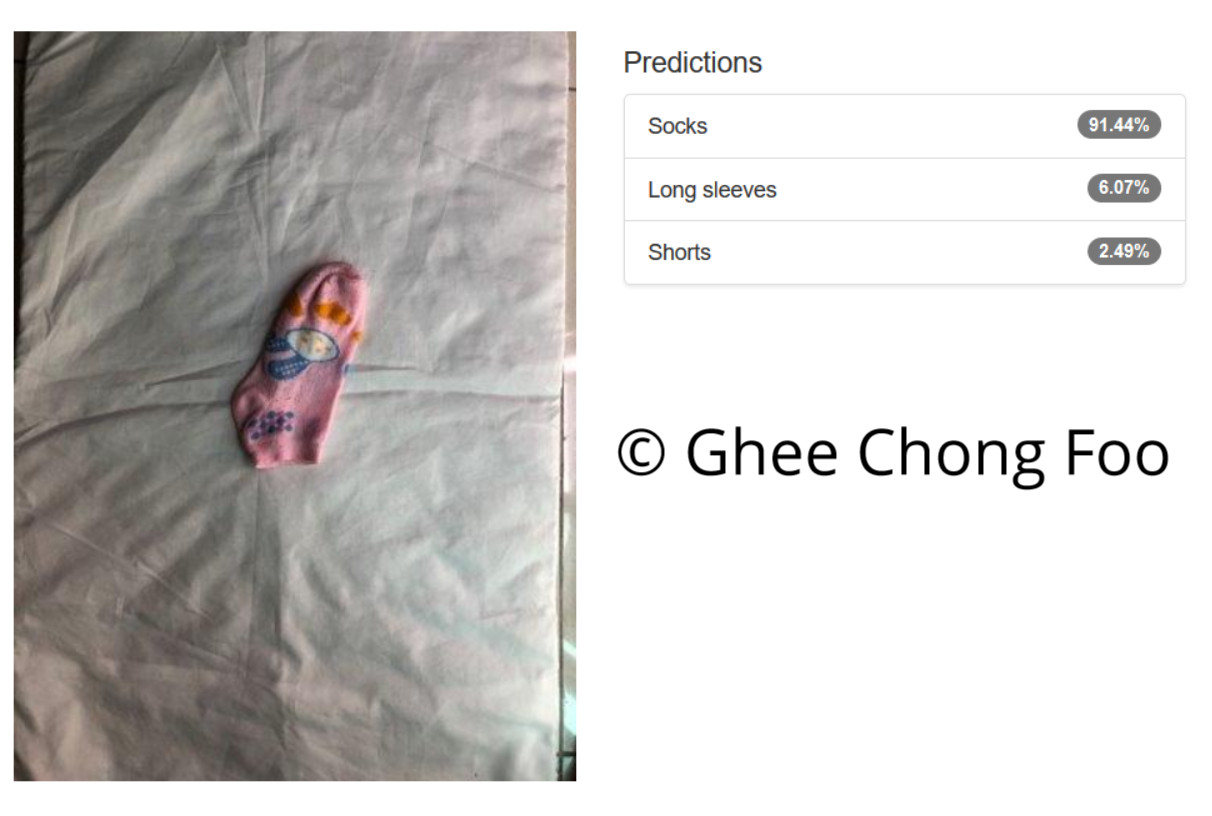
\includegraphics[width=\linewidth]{socks_good_predict1}
      \caption{Good prediction for "Socks" using own data}
      \label{fig:socks_good_predict1}
\end{figure}

% This is typically the hardest part of the report for many. You want to convey your results in an unbiased fashion. If you results are good, you can objectively note this. Similarly, you may do this if they are bad as well. You do not want to justify your results here with discussion; this is a topic for the next session. 
% Present the results of your robotics project model and the model you used for the supplied data with the appropriate accuracy and inference time
% For demonstrating your results, it is incredibly useful to have some charts, tables, and/or graphs for the reader to review. This makes ingesting the information quicker and easier.

\newpage
\section{Discussion}
In this section the result of inference will be discussed, as well as inference time and accuracy between models.

\subsection{Supplied Data}
For supplied data, both AlexNet (4.199ms, 75.4\%) and GoogLeNet (5.04ms, 75.4\%) model meet the project specification of $<$ 10ms and 75\% accuracy.  Hence choosing the model is a trade off between speed and accuracy.  With faster inference time and shorter training time, AlexNet trained model is favored.

\subsection{Own Data}
For own data, predictability is high if model is asked to infer new objects that is acquired in similar setting ($>$90\% accuracy), but performed poorly/unpredictably with images that is downloaded from Internet with different image size, background, as well as style of clothing, from own data.  Since only approximately 1500 images were captured for 3 categories of roughly 500 images each, this suggested that the model accuracy can be further improved if more data was provided during training, some tweaking of hyperparameters, but without much changes needed to the network model.\linebreak

Since the goal of the inference project is to correctly identify the type of cloth and inference time is not critical, \textit{accuracy of inference} take priority over inference time, as consumers would rate accuracy higher than speed.

\subsubsection{Importance of data acquisition}
While data acquisition might be perceived as a mundane task for deep learning, it was found to have huge impact on accuracy of the model.  Initially the image captured was not of similar relative size (i.e. a shirt and socks might have similar size in the image, although shirt normally is much larger than a socks) as images were not captured from a consistent height.  This resulted in poor accuracy and the model did not provide a good prediction.  It was only after the relative size of the object was kept consistent then the predicted accuracy shot up.

\subsubsection{Importance of data processing}
The data acquired need to be processed to suit the model. The default image size captured using smart phone was 3024x4032, which was not optimized for AlexNet that expect input image size of 256x256.  It was only after resizing the image to 360x480, which was much closer to expected image size, then the trained model provided significant improvement on accuracy.  The reduced size of image also reduced the file size significantly, and greatly reduced image upload time when transfered to Amazon S3 bucket and then to DIGITS workspace.  Training time was also significantly reduced with similar accuracy by at least 3x, a critical factor if new model were to be trained with more data.

% faster training speed and upload

% Data collection, keep relative height of image
% Image size for inference, if not result will be unpredictable.  Need larger data set to compensate.



% This is the only section of the report where you may include your opinion. However, make sure your opinion is based on facts. If your results are poor, make mention of what may be the underlying issues. If the results are good, why do you think this is the case? Again, avoid writing in the first person (i.e. Do not use words like “I” or “me”). If you really find yourself struggling to avoid the word “I” or “me”; sometimes, this can be avoid with the use of the word “one”. As an example: instead of : “I think the accuracy on my dataset is low because the images are too small to show the necessary detail” try: “one may believe the accuracy on the dataset is low because the images are too small to show the necessary detail”. They say the same thing, but the second avoids the first person. 
% Reflect on which is more important, inference time or accuracy, in regards to your robotic inference project.

\section{Conclusion / Future work}
Both supplied data and own data have met project specification.  In particular own data portion still have lots of room for improvement as more image sample and categories needs to be captured in order to make this a workable product.  However for the purpose of prototyping it has shown a lot of promise as model was able to accurately classify an object with relatively low number of image samples. \linebreak

Next phase of the project is to design the mechanism to proceed with folding the clothing based on inference result!

% This section is intended to summarize your report. Your summary should include a recap of the results, did this project achieve what you attempted, and is this a commercially viable product? 
% For Future work,address areas of work that you may not have addressed in your report as possible next steps. For future work, this could be due to time constraints, lack of currently developed methods / technology, and areas of application outside of your current implementation. Again, avoid the use of the first-person.

\bibliography{bib}
\bibliographystyle{ieeetr}

\end{document}